\documentclass[./report.tex]{subfiles}
%\documentclass[../../../CR/pac.tex]{subfiles}

\begin{document}

\part{Multiserver Scheduling}

%% ===============================
\section{Principles for the implementation}

In the single server version the \textit{arrivedJobs} list could be used as an \textit{assignedJobs} list. But with multiple servers it became difficult to keep track of which server had started to run each task in the event of a preemption (a task that starts on a server must end on the same server). So we added to the \textit{Server} class an \textit{assignedJobs} list so that each server knows which jobs he has the responsibility of.

\begin{figure}[!h]
	\center
	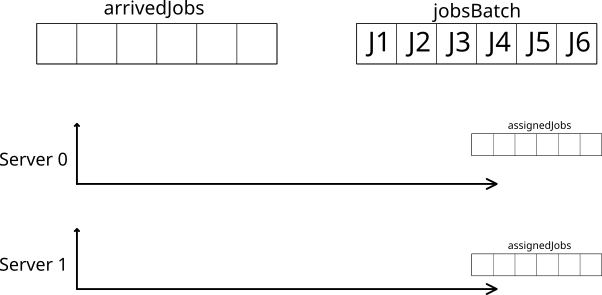
\includegraphics[scale=0.7]{part2/multiServer.png}
	\caption{Initial situation of a multiserver scheduling}
	\label{fig:multiServer_init} 
\end{figure}

In this configuration, jobs from the jobs batch are still by default assigned to the \textit{arrivedJobs} list whenever the current date in the schedule allows it. The method \textit{assignArrivals()} manages the arrival assignments based on the specifications of our algorithms. For example, in EDF, arrived tasks are assigned to a server if:
\begin{enumerate}
	\item The server is idle
	\item The server has a task with a lower priority (ie. lower absolute deadline)\\
\end{enumerate}

If none of these conditions are verified then the task waits in the \textit{arrivedJobs} list. Servers that are idle will fetch the most critical task themselves if they are idle (cf. subsection \ref{subsec:edf} for the corresponding source code).

\newpage
This arrival specification varying from algorithm to algorithm they are redefined in their abstract classes \textit{SchedulerQuantum} and \textit{SchedulerPriority} which consistute families of schedulers\footnote{FIFO and Round Robin corresponding to the \textit{SchedulerQuantum} family and EDF/RMS to the \textit{SchedulerPriority} family}. We provide here an example of an arrival assignment implementation used by the \textit{SchedulerPriority} family:

\begin{lstlisting}[style=Java, caption={Source code of the \textit{assignArrivals()} used by the \textit{SchedulerPriority} family of Schedulers}]
	protected void assignArrivals(Comparator<Job> jobsComparKey, BiPredicate<Job, Job> jobsComparPredicate){
		boolean isAssignable = true;
		boolean isAssigned;
		Iterator<Job> jobIterator = arrivedJ.iterator();
		
		while(jobIterator.hasNext() && isAssignable){
			Job j = jobIterator.next();
			isAssigned = serversM.assignToIdle(j);
			
			if(isAssigned) jobIterator.remove();
			else{
				Server servP = getPreemptable(j, jobsComparPredicate);
				if(servP == null) isAssignable = false;
				else{
					double start = ScheduleEntry.computeStart(schedule, servP, servP.getRunningJob());
					schedule.add(new ScheduleEntry(servP.getRunningJob(), servP, start, schedule.currentDate, servP.getCurrFreq()));
					servP.getAssignedJobs().add(j);
					servP.getAssignedJobs().sort(jobsComparKey);
					jobIterator.remove();
				}
			}
		}
	}
\end{lstlisting}
 
%% ===============================
\newpage
\section{EDF}
\subsection{Implementation}
The algorithm used is the same as presented in subsection \ref{subsec:edf} of the previous part of this report.

\subsection{Scheduling results}
\begin{figure}[!h]
	\center
	\includegraphics[scale=0.5]{test_multiServer_edf.png}
	\caption{Output schedule produced by the EDF scheduling algorithm on multiple servers}
	\label{fig:multiServer_edf} 
\end{figure}

Which corresponds to following file (<jobID, serverID, startDate, endDate, frequency>):
\lstinputlisting[style=txt, caption={Detail of the scheduling result}]{test_multiServer_edf.txt}

\newpage
\subsection{Metrics}
\begin{lstlisting}[style=txt, caption={Metrics for EDF on multiple servers}]
################ SCHEDULE METRICS ################

>> Scheduling Metrics: 
- Total Makespan: 126.0
- Nb Deadline Misses: 0
- Max Tardiness: 0.0
- Average Tardiness: 0.0
- Late Jobs: 

>> Servers Metrics: 
- Servers work load:
Server #0 : 55.0
Server #1 : 31.0
Server #2 : 25.0
Server #3 : 15.0

>> Energy Metrics: 
- Total Consumption: 4077.777777777775
- Max Consumption: 144.44444444444446
- Average Consumption: 1019.4444444444438
- Consumption per Server: 
Server #0 : 1222.2222222222208
Server #1 : 1550.0
Server #2 : 555.5555555555555
Server #3 : 750.0

##################################################
\end{lstlisting}


%% ===============================
\newpage
\section{RMS}
\subsection{Implementation}
The algorithm used is the same as presented in subsection \ref{subsec:rms} of the previous part of this report.

\subsection{Scheduling results}
\begin{figure}[!h]
	\center
	\includegraphics[scale=0.5]{test_multiServer_rms.png}
	\caption{Output schedule produced by the RMS scheduling algorithm on multiple servers}
	\label{fig:multiServer_rms} 
\end{figure}

Which corresponds to following file (<jobID, serverID, startDate, endDate, frequency>):
\lstinputlisting[style=txt, caption={Detail of the scheduling result}]{test_multiServer_rms.txt}

\newpage
\subsection{Metrics}
\begin{lstlisting}[style=txt, caption={Metrics for RMS on multiple servers}]
################ SCHEDULE METRICS ################

>> Scheduling Metrics: 
- Total Makespan: 126.0
- Nb Deadline Misses: 1
- Max Tardiness: 6.0
- Average Tardiness: 6.0
- Late Jobs: 
[Job: J8{11.0a/0.0u/5.0rd/16.0ad/0.0p} | Tardiness: 6.0 ]

>> Servers Metrics: 
- Servers work load:
Server #0 : 65.0
Server #1 : 17.0
Server #2 : 25.0
Server #3 : 19.0

>> Energy Metrics: 
- Total Consumption: 3799.999999999997
- Max Consumption: 144.44444444444446
- Average Consumption: 949.9999999999992
- Consumption per Server: 
Server #0 : 1444.4444444444425
Server #1 : 850.0
Server #2 : 555.5555555555555
Server #3 : 950.0

##################################################
\end{lstlisting}


%% ===============================
\newpage
\section{Comparison Table}

\begin{tabular}{|m{8em}|m{12em}|m{12em}|m{12em}|} 
	\hline 
	\textbf{Algorithm} & \textbf{Pros} & \textbf{Cons} & \textbf{Possible Uses} \\ 
	\hline
	EDF 
	&  
	\begin{itemize}[leftmargin=*]
		\item With several servers (or cores): lowest number of deadline misses and lowest average tardiness
		\item Best workload share among servers
	\end{itemize}
	&  
	\begin{itemize}[leftmargin=*]
		\item What if the deadline is superior to the period of the task?
		\item Rather hard to implement and maintain on several servers (lot of lists sorting)
	\end{itemize}
	& 
	\begin{itemize}[leftmargin=*]
		\item May be the best algorithm for hard real time OS if the deadline is inferior to the period of the task
	\end{itemize}
	\\
	\hline
	RMS 
	& 
	\begin{itemize}[leftmargin=*]
		\item Very low number of deadline misses and average tardiness
	\end{itemize} 
	&  
	\begin{itemize}[leftmargin=*]
		\item Rather hard to implement for the same reasons than with EDF
		\item Not the best algorithm for hard real time OS if the deadline of the tasks is inferior to their periods?
	\end{itemize}
	& 
	\begin{itemize}[leftmargin=*]
		\item May still be the best algorithm for hard real time OS if tasks' deadlines are equal or superior to their periods
	\end{itemize}
	\\
	\hline
\end{tabular}

\end{document}